\documentclass[bachelor]{njupthesis}

\title{定向覆盖模糊测试工具的设计与实现}
\author{雷尚远}
\advisor{王子元}
\school{计算机学院、软件学院、网络空间安全学院}
\major{计算机科学与技术}
\studentclass{B190303}
\studentid{B19030334}
\graduateyear{2023}
\begindate{2023年3月x日}
\finishdate{2023年6月x日}


\begin{document}

\makecover

\begin{chineseabstract}
模糊测试(Fuzzing)是一种通过向目标系统提供非预期的输入并监视异常结果来发现软件安全漏洞的方法,
是软件安全领域常用的方法之一。由于代码覆盖率与漏洞覆盖率密切相关,大多数模糊测试工具都是
以代码覆盖率为导向。然而,由于大多数被覆盖测试的代码可能并不包含漏洞,这使得盲目地扩展
代码覆盖率的方式在实际测试时效率较低。极端情况尤为如此。与盲目增加代码覆盖率的模糊测试不同,
定向覆盖的灰盒模糊测试(DGF)将大部分时间用于检测特定目标区域(例如,易出错代码段)而不会
浪费资源于不相关的部分。因此,DGF 特别适用于补丁测试、漏洞复现以及特殊漏洞检测等场景。
目前,DGF 已成为一个快速发展的研究方向。基于一些先进的定向覆盖模糊测试工具的研究和相关调查,本文
主要做了以下点工作:
\begin{enumerate}[label=(\arabic*)]
	\item 基于现有的模糊测试工具框架AFL(American Fuzzy Lop)以及AFLGo做了定向覆盖策略的设计和集成;
	\item 实现了简单的定向覆盖的模糊测试命令行工具;
	\item 针对相应的公开通用漏洞集(CVE)做了复现及定向实验对比测试。
\end{enumerate}
此外本文亦通过分析工具设计以及实现过程中的局限性与不足,对于未来该方向的研究发展做出了一些展望。

\chinesekeyword{模糊测试;定向覆盖模糊测试;灰盒测试;软件安全}
\end{chineseabstract}

\begin{englishabstract}
Fuzzing is a method of discovering software security vulnerabilities by providing 
unexpected inputs to a target system and monitoring for abnormal results. It is one of the 
commonly used methods in the field of software security. As code coverage is closely related 
to vulnerability coverage, most fuzz testing tools are guided by code coverage. However, blindly 
extending code coverage may be inefficient in practical testing since most of the covered code 
may not contain vulnerabilities, especially for corner cases.  In contrast to blind code coverage-based 
fuzz testing, directed grey-box fuzzing (DGF) spends most of its time detecting specific target regions 
(such as error-prone code segments) rather than wasting resources on irrelevant parts. 
Thus, DGF is particularly suitable for scenarios such as patch testing, bug reproduction, and 
special bug detection. For now, DGF has become a fast-growing research area.  Based on some advanced 
directed coverage fuzz testing tools and relevant investigations, this article mainly focuses on the 
following points of work:
\begin{enumerate}[label=(\arabic*)]
	\item Designed and integrated a directed coverage strategy based on the existing fuzzy testing tool framework AFL (American Fuzzy Lop) and AFLGo;
	\item Implemented a simple command-line tool for directed fuzz testing;
	\item conducted reproductions and directed experiments on corresponding public vulnerability databases (CVE) for comparative testing。
\end{enumerate}
In addition, this article also provides some prospects for the future research and development of this direction by 
analyzing the limitations and deficiencies in the design and implementation process of the tool.


\englishkeyword{Fuzzing;Directed Greybox Fuzzing;Greybox test;Software Security}
\end{englishabstract}

\thesistableofcontents

\thesischapterexordium

\chapter{绪论}
\section{背景分析}
“常用系统中可能会潜伏着严重的漏洞\cite{miller1990empirical}。”这一论述源自于模糊测试首次面世的论文。其
揭示了一个事实,即随着软件技术的不断发展,软件安全问题就将日益成为愈发重视的议题。在当前的信息化时代,
软件已经成为了人们生活、工作和娱乐的重要组成部分,这也意味着我们将面临着越来越多的安全威胁。
因此,确保软件安全已经成为了一项非常重要的任务。

软件安全(Software Security)就是使软件在受到恶意攻击的情形下依然能够继续正确运行及确保软件被在授权范围
内合法使用的思想。在当今社会,软件越来越普及,并被广泛应用于各个领域,包括电商、金融、医疗等。但是,
由于软件的复杂性和开发过程中的缺陷,软件本身也存在着各种安全问题。这些问题可能导致信息泄露、数据损坏、远程攻击等,
对个人、企业甚至整个社会造成巨大的损失。因此,保障软件安全显得尤为重要。

近年来,因为软件漏洞造成的损失案例屡见不鲜。2017年,全球范围内爆发了 WannaCry 勒索病毒攻击事件,
该攻击利用了微软 Windows 操作系统中的漏洞,并导致了数十亿美元的经济损失;2019年,美国资讯技术服务公司 SolarWinds 
遭受了一次大规模的网络攻击,该攻击利用了 SolarWinds Orion 平台软件中的漏洞,影响了包括
美国联邦政府在内的许多组织和机构;2021年2月,法国LCL银行的客户登录自己的银行应用程序时,
看到的是别人的银行账户信息。原因是由于备份超级计算机系统(日本惠普公司制造)的程序存在缺陷,超级计算机系统出现
了意外,其中存储(/ LARGE0)中的某些数据被误删除;2021年12月,知名日志框架Log4j2被爆出远程代码执行漏洞,
影响了大量使用该框架的中间件和应用,给企业和用户带来了巨大的安全风险。

以上诸多例子可以说明,大多数的安全事件都是攻击者利用软件系统中的漏洞从而进行攻击引发的。因而可以帮助发现和
修复安全漏洞的软件测试技术(Software testing)一直以来都是是软件安全领域的一个重要议题。

软件测试可以通过模拟攻击者的行为来发现这些安全漏洞,并提供关于如何修复这些漏洞的信息。例如,
黑盒测试可以探测应用程序中的安全问题,白盒测试可以评估应用程序的源代码中是否有漏洞,
静态分析可以扫描源代码以发现潜在的安全问题,动态分析可以模拟攻击场景并检查应用程序的反应。

此外,软件测试还可以帮助确保应用程序在面对各种攻击时具有足够的鲁棒性和可靠性。它可以测试应用程序的
身份验证和授权机制、加密技术、网络协议、输入输出数据验证等方面的功能,以确保应用程序满足安全需求。

\section{国内外研究现状}
软件安全信息系统和软件安全代码的有效安全项目往往依靠两种自动的安全测试:静态安全扫描测试和动态安全扫描测试。

在软件的开发期间,为了保证软件的安全性,通常会进行软件安全静态扫描。这个过程是通过威胁建模和分析来完成的,
其目的是对静态代码进行全面地扫描,以便及早地发现任何可能存在的安全漏洞。其是在不运行程序的情况下对软件
进行测试和评估。静态分析可以检查代码、设计和文档等,以发现潜在的问题和错误,并确保软件符合某些标准或规范。由于本文
主要探讨针对代码的漏洞审查,关于软件工程部分的文档、标准以及接口设计的测试技术在此不再赘述。利用数据流分析,符号执行
以及污点分析等静态软件分析技术可以检查源代码中的错误和缺陷,包括语法错误、类型错误、内存泄漏、空指针引用等。
与传统的动态测试相比,静态扫描可以更早地发现安全问题,因为它可以在代码尚未被编译或执行之前就进行检测。
此外,静态扫描还可以减少测试成本,提高测试效率,并帮助开发团队更好地理解代码中的潜在安全风险。

软件安全动态扫描是一种对工作环境中实际运行的代码进行扫描的技术,它能够在代码运行时检测和分析可能存在的漏洞、
缺陷和错误。与静态代码分析不同,动态扫描具有更强的准确性和实时性,因为它是在真实的环境中对代码进行测试和评估。
通过使用动态扫描技术,开发人员和安全专家可以有效地识别并修复潜在的安全漏洞,从而保护软件系统免受攻击和破坏。
此外,动态扫描还可以帮助企业遵循各种合规性标准和法规要求,确保其软件应用程序的安全性和稳定性。

模糊测试技术(Fuzzing Test)是动态安全扫描测试中重要的一种方式。而自从1988年模糊测试这一概念被提出后,
这一方法一直在软件安全测试领域保持着较高的活跃度和关注度。在提出伊始,其主要用于测试操作系统。之后,随着软件技术的发展,
模糊测试技术不断得到改进和推广,并应用于网络、移动设备等领域。目前,模糊测试技术已成为一种成熟的自动化测试技术,
可以有效地检测软件中存在的漏洞和安全隐患。并且迄今为止其社区依然十分活跃,在GitHub上有超过1000个与模糊测试相关的仓库\cite{manes2019art}。
为了防止被恶意攻击,许多商业软件公司,例如Adobe, Cisco, Google, 和Microsoft都将模糊测试作为其雇员软件开发安全测试的必要环节。
可以说,模糊测试是软件安全领域中一个经久不衰的热门议题。

而定向模糊测试(Directed Fuzzing)作为模糊测试的一个研究方向,主要关注重点区域(例如, 易出错区域) 并且将大
部分的时间用于到达测试这些位置而不浪费资源在无关部分\cite{wang2022}。从本源上讲, 定向模糊测试工具早期的解决思路
主要是基于利用程序分析和约束求解来生成检测不同程序执行路径输入符号的执行技术
\cite{ganesh2009taint,ma2011directed,person2011directed,do2013dynamic,ge2011dyta,li2013software}。
然而, 由于定向符号执行技术(DSE) 依赖于大量的程序分析和约束求解, 其受限于兼容性和可扩展性的限制。

在2017 年, Böhme等人引入了定向灰盒模糊测试(DGF)的概念\cite{bohmeDGF2017}。这是定向模糊测试的又一重要工作。
其开创式地将将位置的可达性问题转化为生成种子和其目标集之间距离的最小值问题。通过给更靠近目标集的种子更多的变异机会, 它可
以逐渐引导灰盒测试接近程序目标位置。与定向符号执行技术相比, DGF有更好的可拓展性,并且在测试效率上有几个数量级的提升。
例如, Böhme 等人可以在20 分钟内重现 Heartbleed\cite{Heartbleed}(CVE-2014-0160)漏洞, 而定向符合执行工具
KATCH\cite{marinescu2013katch} 需要24 小时以上\cite{bohmeDGF2017}。

此后,许多针对于

\section{研究内容}
\section{论文结构}

\chapter{相关技术研究}
\section{模糊测试技术}
\subsection{黑盒模糊测试技术}
\subsection{白盒模糊测试技术}
\subsection{灰盒模糊测试技术}
\section{定向模糊测试技术}
\subsection{白盒定向模糊测试技术}
\subsection{灰盒定向模糊测试技术}
\section{研究动机}
\section{本章小结}

\chapter{定向模糊测试策略设计}
\section{AFLGo架构研究}
\subsection{距离计算机制}
\subsection{能量调度机制}
\section{定向适应度指标}
\subsection{距离定义}
\subsection{目标函数集覆盖率}
\subsection{能量调度机制}
\section{本章小结}


\chapter{基于AFLGo的定向模糊测试系统的实现}
\section{需求分析}
\section{架构设计}
\section{静态分析器的改进}
\section{定向模糊测试工具}
\section{本章小结}

\chapter{系统测试}
\section{系统测试概述}
\subsection{系统测试目标}
\subsection{系统测试环境}
\section{功能测试}
\section{实验评估}
\subsection{定向模糊测试工具}
\section{本章小结}


\chapter{总结与展望}
\section{总结}
\section{展望}

% \section{Apple M1}
% 这是一个公式
% \begin{equation}
% 	y=A x+b
% \end{equation}


% \subsection{名字自己替换}
% 1994年12月,中国国务院批准开展京沪高速铁路预可行性研究。铁道部开展京沪高铁选线,提出“北线方案”,即从上元门地区,通过隧道过江。南京的规划部门则拿出“南线方案”,从大胜关过江。铁道部牵头,进行比选得出的结论是:两个方案在技术上都可行,主要差别在于工程造价、经济效益、运营条件等方面。江苏省和南京市要求南线方案,而铁道部看好的始终是北线方案。南京力主南线,是放长了眼光。如果从南京北部走,已经不具备扩建条件。南京火车站虽然前面是玄武湖、背面是小红山,景观很美,但是已经没有拓展空间。此外,更重要的是,在全国任何一个城市,铁路带动城市发展的效果都非常明显,南京要想进一步发展南部区域,这是个好机会。显然,高铁建在哪里,也就意味着南京今后的发展框架,是继续囿于老城狭小的空间里,还是大步向南拓展。铁道部青睐北线的理由:新线与既有线的衔接方便。清末修建的津浦铁路,即从天津到浦口;在长江南岸,之后又修建了沪宁铁路。浦口火车站、下关火车站、南京站,南京重要的火车站,向来都是位于城北。并且,当时铁道部的人都认为,南京的城市中心就在北边。另一方面,铁路的机务段、职工宿舍等都在城北,建成之后,职工上下班都方便。为了说服铁道部,南京方面列出了南线的九大优势:无论高铁从哪里走,从完善南京枢纽总体布局的角度来看,都必须建大胜关长江大桥;根据国务院批准的南京城市规划,南京城市今后将主要向东南方向发展,大胜关方案符合城市扩展方向;南面的场站位置已预留多年,有较为理想的建站条件;沿线拆迁量小,对城市干扰和环境影响小;利于形成方便的铁路——航空换乘及铁路与城市道路联结条件……不过,这些最初并没有打动铁道部,铁道部仍然坚持北线方,双方为此对峙了好几年。


% \subsection{名字自己替换}
% 1995年,为了促进高铁尽快上马,南京稍稍“松口”。在当年的一份紧急报告里,有这样一句话——“南北方案之争不宜过多坚持,而从规划上对北线方案提出完善意见为妥”。南京市规划局做了两手准备,针对南线、北线方案,分别做了规划控制。从1995年起,南京根据两个方案,开始分别严格控制沿线用地建设,同时冻结了南北两条线周围的土地。而这个具有预见性的做法,使得后来的工作变得轻松许多。

% 南京南站如图\ref{南京南站}所示。
% \begin{figure}[hbt]
% 	\centering
% 	\subfigure[南京南1]{
% 		\begin{minipage}[b]{0.4\textwidth}
% 			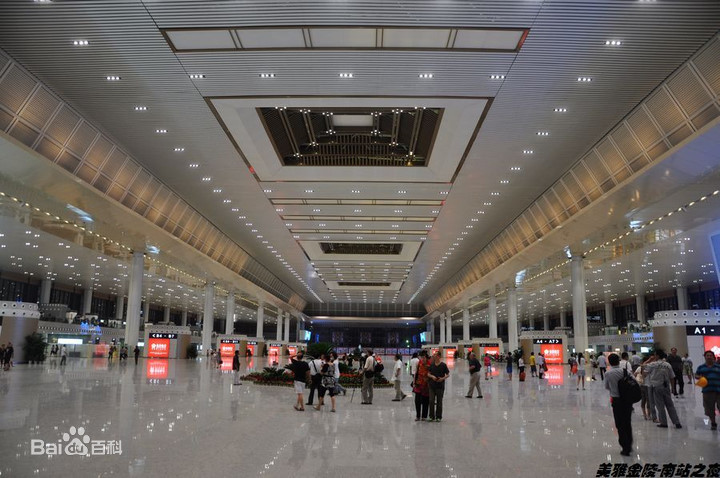
\includegraphics[width=1\textwidth]{1}
% 		\end{minipage}
% 	}
% 	\subfigure[南京南2]{
% 		\begin{minipage}[b]{0.4\textwidth}
% 			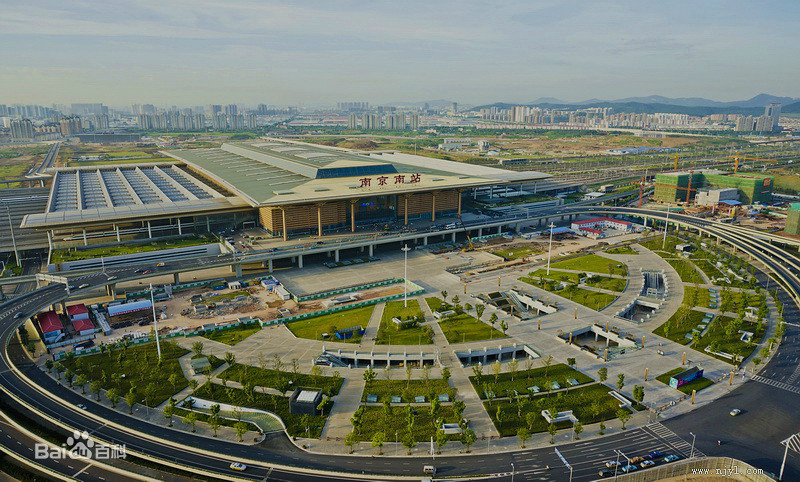
\includegraphics[width=1\textwidth]{2}
			
% 		\end{minipage}
% 	} \\
% 	\subfigure[南京南3]{
% 		\begin{minipage}[b]{0.4\textwidth}
% 			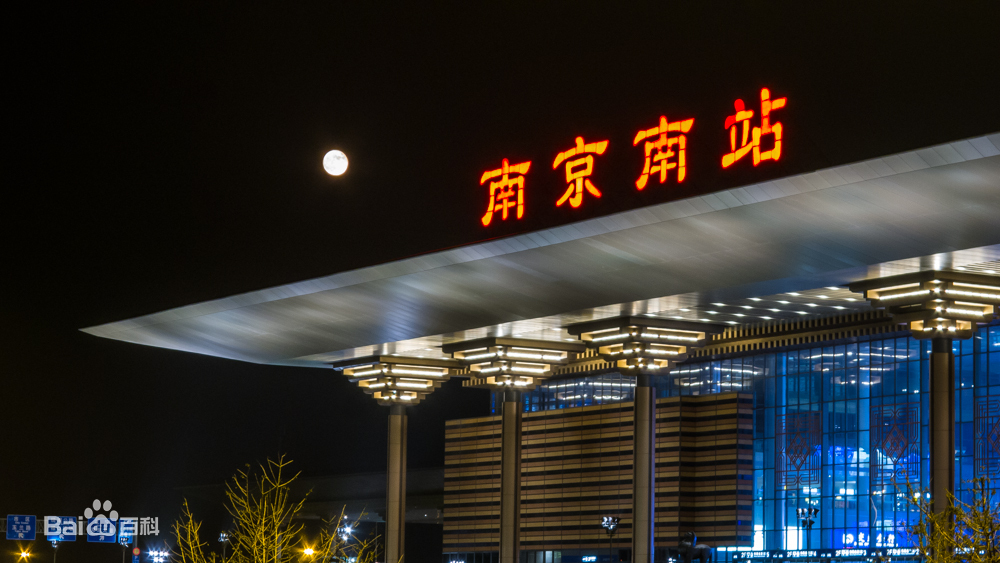
\includegraphics[width=1\textwidth]{3}
% 		\end{minipage}
% 	}
% 	\subfigure[南京南4]{
% 		\begin{minipage}[b]{0.4\textwidth}
% 			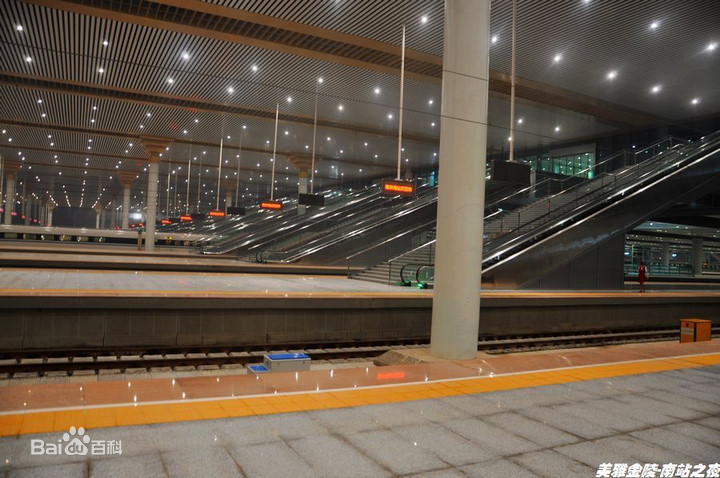
\includegraphics[width=1\textwidth]{4}
			
% 		\end{minipage}
% 	}
% 	\caption{南京南站}
% 	\label{南京南站}
% \end{figure}

%这里是结束语
\thesisconclusion

% 致谢区域
\thesisacknowledgement

本论文采用\LaTeX 模版编写的,是基于南京邮电大学2021年理工艺教类的Word模板进行严格迁移编写的。本模板地址\url{https://github.com/dhiyu/NJUPT-Bachelor}感谢imguozr(\url{https://github.com/imguozr/NJUPThesis-Bachelor} )和lemoxiao(\url{https://github.com/lemoxiao/NJUPThesis-Scholar} )的工作,为本模板的形成奠定了大量的基础。

% 参考文献区域
\thesisreference

\end{document}